\documentclass[12pt]{standalone}
\usepackage{tikz}
\usetikzlibrary{positioning}
\begin{document}
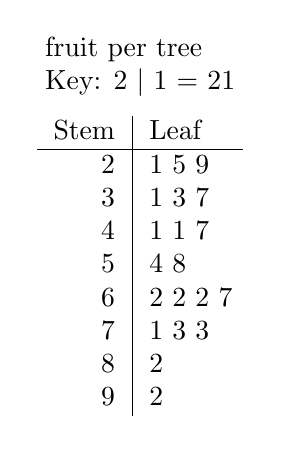
\begin{tikzpicture}
\node[align=left] (top_node) at (0,0){fruit per tree \\ Key: 2 $\vert$ 1 = 21};
\node[below=of top_node,yshift=10mm] {
\begin{tabular}{r|l@{\hspace{4 pt}}}
Stem & Leaf\\
\hline
2 & 1 5 9 \\3 & 1 3 7 \\4 & 1 1 7 \\5 & 4 8 \\6 & 2 2 2 7 \\7 & 1 3 3 \\8 & 2 \\9 & 2 \\
\end{tabular}};
\end{tikzpicture}
\end{document}